\documentclass[
	12pt,				% tamanho da fonte
	oneside,			% para impressão em recto e verso. Oposto a oneside
	a4paper,			% tamanho do papel. 
	english,			% idioma adicional para hifenização
	brazil,				% o último idioma é o principal do documento
	]{abntex2}

% ---
% Pacotes fundamentais 
% ---
\usepackage{lmodern}			% Usa a fonte Latin Modern
\usepackage[T1]{fontenc}		% Selecao de codigos de fonte.
\usepackage[utf8]{inputenc}		% Codificacao do documento (conversão automática dos acentos)
\usepackage{indentfirst}		% Indenta o primeiro parágrafo de cada seção.
\usepackage{color}				% Controle das cores
\usepackage{graphicx}			% Inclusão de gráficos
\usepackage{microtype} 			% para melhorias de justificação
\usepackage{multicol}
\usepackage{multirow}
\usepackage[brazilian,hyperpageref]{backref}	 % Paginas com as citações na bibl
\usepackage[alf]{abntex2cite}	% Citações padrão ABNT
\usepackage{listings}
\usepackage{float}

\lstset{
  showspaces=false,
  showtabs=false,
  breaklines=true,
  showstringspaces=false,
  breakatwhitespace=true,
  commentstyle=\color{green},
  keywordstyle=\color{blue},
  stringstyle=\color{red},
  basicstyle=\ttfamily
}

% --- 
% CONFIGURAÇÕES DE PACOTES
% --- 

% ---
% Configurações do pacote backref
% Usado sem a opção hyperpageref de backref
\renewcommand{\backrefpagesname}{Citado na(s) página(s):~}
% Texto padrão antes do número das páginas
\renewcommand{\backref}{}
% Define os textos da citação
\renewcommand*{\backrefalt}[4]{
	\ifcase #1 %
		Nenhuma citação no texto.%
	\or
		Citado na página #2.%
	\else
		Citado #1 vezes nas páginas #2.%
	\fi}%
% ---

% ---
% Informações de dados para CAPA e FOLHA DE ROSTO
% ---
\titulo{Prática 8: APIs REST}
\autor{Pedro Inácio Rodrigues Pontes}
\local{Belo Horizonte, Brasil}
\data{2025}
\instituicao{%
  Universidade Federal de Minas Gerais
  \par
  Colégio Técnico
  \par
  Curso Técnico em Desenvolvimento de Sistemas}

\definecolor{blue}{RGB}{41,5,195}

\makeatletter
\hypersetup{
     	%pagebackref=true,
		pdftitle={\@title}, 
		pdfauthor={\@author},
    	pdfsubject={\imprimirpreambulo},
		colorlinks=true,       		% false: boxed links; true: colored links
    	linkcolor=blue,          	% color of internal links
    	citecolor=blue,        		% color of links to bibliography
    	filecolor=magenta,      		% color of file links
		urlcolor=blue,
		bookmarksdepth=4
}
\makeatother

\renewcommand{\thesection}{\arabic{section}}
\setlength{\parindent}{1.3cm}
\setlength{\parskip}{0.2cm} 

\makeindex


\begin{document}

\selectlanguage{brazil}
\frenchspacing 

\imprimircapa

{
\ABNTEXchapterfont

\textual

% ----------------------------------------------------------
% Introdução (exemplo de capítulo sem numeração, mas presente no Sumário)
% ----------------------------------------------------------
\section{Introdução}

O objetivo deste projeto é desenvolver um programa de console em C# que realize o monitoramento contínuo de temperatura através de requisições periódicas a um serviço REST local. O programa deve solicitar ao usuário a unidade de temperatura desejada (Celsius, Kelvin ou Fahrenheit) e o intervalo em segundos para cada nova leitura, realizando então requisições HTTP GET ao endpoint http://localhost:5000/temperatura/{unidade} em intervalos regulares. A cada resposta bem-sucedida, o sistema deve capturar o horário local exato, comparar o valor atual com a leitura anterior para determinar se a temperatura subiu, desceu ou permaneceu igual, e apresentar essas informações no console com formatação colorida: vermelho para indicar aumento de temperatura, azul para diminuição e cor padrão para ausência de alteração. O programa deve incluir tratamento robusto de erros para requisições HTTP falhadas ou respostas JSON inválidas, exibindo mensagens apropriadas em cor amarela, e permitir interrupção controlada pelo usuário através de comandos como Ctrl+C, finalizando com uma mensagem de encerramento adequada.

\section{Desenvolvimento}

\subsection{RestServer}
Esta classe foi fornecida pronta pelo professor e representa um servidor REST simples que simula leituras de temperatura. O servidor utiliza o framework ASP.NET Core para criar um endpoint HTTP que retorna valores de temperatura calculados matematicamente com base no horário atual, simulando variações realistas ao longo do dia.

\begin{itemize}
    \item \textbf{Construtor RestServer}
    Inicializa o servidor web através do \textit{WebApplicationBuilder} e configura o endpoint \texttt{/temperatura/\{unidade\}}. O endpoint aceita requisições GET onde o parâmetro \textit{unidade} especifica a escala de temperatura desejada (celsius, kelvin ou fahrenheit).
    
    \item \textbf{Algoritmo de Simulação}
    A temperatura base é calculada usando uma função senoidal que varia entre 20°C e 30°C ao longo de 24 horas, simulando o ciclo natural de temperatura diária. A fórmula utilizada é: \texttt{25.0 + 5.0 * Sin((2π/24) * hora\_atual)}. Um componente de ruído aleatório é adicionado para tornar as leituras mais realistas.
    
    \item \textbf{Conversão de Unidades}
    O servidor suporta três unidades de temperatura:
    \begin{itemize}
        \item Celsius: valor base (sem conversão)
        \item Kelvin: temperatura em Celsius + 273.15
        \item Fahrenheit: (temperatura em Celsius × 9/5) + 32
    \end{itemize}
    
    \item \textbf{Método StartAsync}
    Inicia o servidor de forma assíncrona, permitindo que ele aceite requisições HTTP na porta configurada (padrão 5000).
    
    \item \textbf{Resposta JSON}
    Retorna um objeto JSON contendo a unidade solicitada e o valor da temperatura arredondado para duas casas decimais. Em caso de unidade inválida, retorna um erro HTTP 400 (Bad Request).
\end{itemize}

\subsubsection{Demonstração}
Estrutura da classe RestServer:
\begin{lstlisting}[language=csharp]
public class RestServer
{
    WebApplicationBuilder builder;
    WebApplication app;
    
    public RestServer(string[]? args = null)
    {
        // Configuração do servidor e endpoint
    }
    
    public async void StartAsync()
    {
        // Inicialização assíncrona do servidor
    }
}
\end{lstlisting}

\subsection{Temperatura}
Esta classe representa um modelo de dados simples (DTO - Data Transfer Object) criado especificamente para deserializar a resposta JSON retornada pelo servidor REST. Ela serve como uma estrutura de mapeamento entre o formato JSON recebido nas requisições HTTP e os objetos C# utilizados pelo programa cliente.

\begin{itemize}
    \item \textbf{Propriedade unidade}
    Propriedade do tipo \textit{string} nullable que armazena a unidade de temperatura retornada pelo servidor (celsius, kelvin ou fahrenheit). O uso de tipo nullable permite tratamento adequado de respostas JSON incompletas ou malformadas.
    
    \item \textbf{Propriedade valor}
    Propriedade do tipo \textit{double} nullable que contém o valor numérico da temperatura na unidade especificada. O tipo nullable oferece flexibilidade para lidar com cenários onde o valor pode estar ausente na resposta JSON.
    
    \item \textbf{Padrão de Propriedades Automáticas}
    Ambas as propriedades utilizam o padrão de propriedades automáticas com getters e setters públicos, facilitando a serialização/deserialização automática pelo sistema de JSON do .NET.
\end{itemize}

\subsubsection{Demonstração}
Estrutura da classe Temperatura:
\begin{lstlisting}[language=csharp]
public class Temperatura
{
    public string? unidade { get; set; }
    public double? valor { get; set; }
}
\end{lstlisting}

\subsection{Program}
Esta classe representa o ponto de entrada da aplicação e implementa toda a lógica principal do programa de monitoramento de temperatura. É responsável por coordenar a inicialização do servidor, configuração dos parâmetros de monitoramento, execução do ciclo de requisições periódicas e tratamento da interrupção controlada pelo usuário.

\begin{itemize}
    \item \textbf{Propriedades Estáticas}
    A classe utiliza propriedades estáticas para armazenar o estado global da aplicação: \textit{UnidadeDesejada} (string para a unidade de temperatura), \textit{IntervaloDeRequisicao} (int para o intervalo em segundos), \textit{Url} (string para o endpoint construído) e \textit{AnteriorTemp} (double nullable para comparação entre leituras).
    
    \item \textbf{Método Main}
    Ponto de entrada assíncrono que coordena toda a execução do programa. Inicializa o servidor REST local, configura o tratamento de interrupção via Ctrl+C usando \textit{CancellationTokenSource}, realiza a validação das entradas do usuário (unidade e intervalo), constrói a URL do endpoint e executa o loop principal de monitoramento até que seja cancelado.
    
    \item \textbf{Método ExibirTemperatura}
    Método assíncrono responsável por executar uma única iteração do ciclo de monitoramento. Realiza a requisição HTTP GET ao servidor, deserializa a resposta JSON usando \textit{JsonSerializer}, compara o valor atual com a temperatura anterior para determinar a tendência (subida, descida ou estabilidade), atualiza o estado da temperatura anterior e exibe o resultado formatado no console com timestamp e símbolos indicativos.
    
    \item \textbf{Tratamento de Cancelamento}
    Implementa um sistema robusto de cancelamento baseado em \textit{CancellationToken}, permitindo interrupção controlada tanto pelo usuário (Ctrl+C) quanto por exceções do sistema, garantindo que o programa finalize adequadamente em todas as situações.
    
    \item \textbf{Validação de Entrada}
    Inclui validação básica dos parâmetros fornecidos pelo usuário, verificando se a unidade de temperatura está entre as opções válidas (celsius, fahrenheit, kelvin) e se o intervalo de requisição é um valor não-negativo.
\end{itemize}

\subsubsection{Demonstração}
Estrutura da classe Program com trechos importantes:
\begin{lstlisting}[language=csharp]
public class Program
{
    static string? UnidadeDesejada { get; set; }
    static int IntervaloDeRequisicao { get; set; }
    static string? Url { get; set; }
    static double? AnteriorTemp { get; set; }
    
    public static async Task Main(string[] args)
    {
        RestServer server = new();
        server.StartAsync();
        
        using var cts = new CancellationTokenSource();
        Console.CancelKeyPress += (sender, e) =>
        {
            e.Cancel = true;
            cts.Cancel();
            Console.WriteLine("\nParando o monitoramento...");
        };
        
        [...]
        if (UnidadeDesejada != "celsius" && UnidadeDesejada != "fahrenheit" && UnidadeDesejada != "kelvin")
        {
            Console.WriteLine("Selecione uma unidade válida");
            return;
        }
        
        [...]
        while (!cts.Token.IsCancellationRequested)
        {
            await ExibirTemperatura(httpClient, cts.Token);
        }
    }
    
    static async Task ExibirTemperatura(HttpClient httpClient, CancellationToken cancellationToken)
    {
        HttpResponseMessage response = await httpClient.GetAsync(Url, cancellationToken);
        string jsonString = await response.Content.ReadAsStringAsync();
        var temperatura = JsonSerializer.Deserialize<Temperatura>(jsonString);
        
        [...]
        if (temperatura.valor > AnteriorTemp)
        {
            symbol = "↑";
        }
        else if (temperatura.valor < AnteriorTemp)
        {
            symbol = "↓";
        }
        
        Console.WriteLine($"[{DateTime.Now:HH:mm:ss}]Temperatura: {temperatura.valor}°{temperatura.unidade} {symbol}");
        await Task.Delay(IntervaloDeRequisicao * 1000, cancellationToken);
    }
}
\end{lstlisting}

\section{Resultados}

\begin{figure}[H]
    \centering
    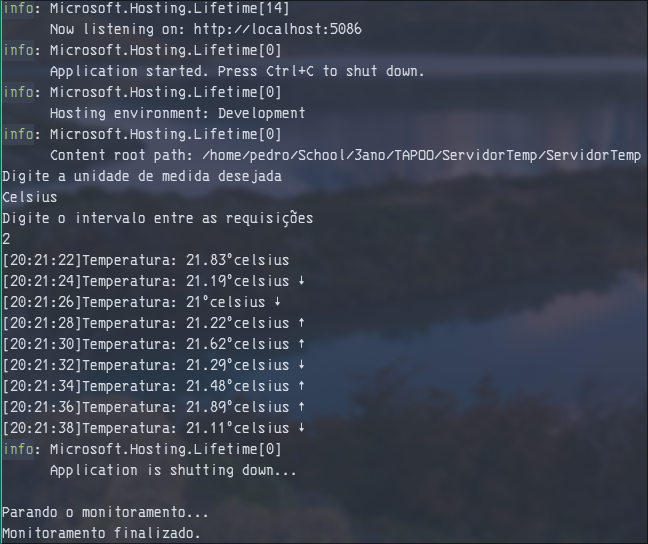
\includegraphics[width=1\textwidth]{imgs/img1.png}
    \caption{Execução do programa com unidade Celsius}
    \label{fig:img1}
\end{figure}

\begin{figure}[H]
    \centering
    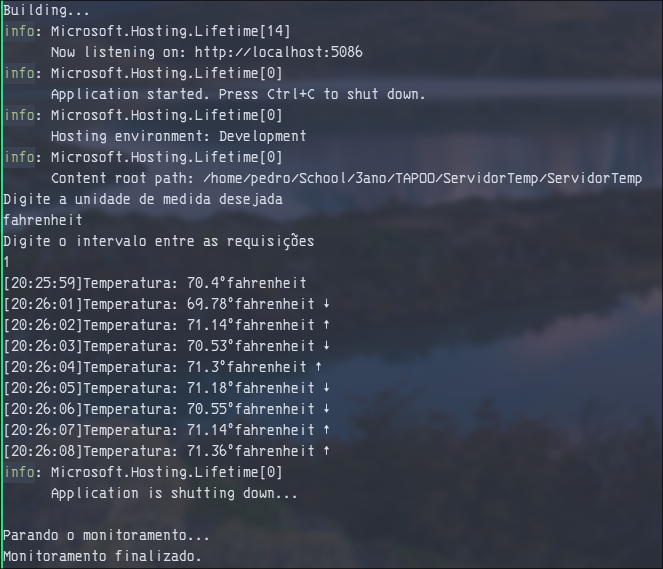
\includegraphics[width=1\textwidth]{imgs/img2.png}
    \caption{Execução do programa com unidade Fahrenheit}
    \label{fig:img2}
\end{figure}

\begin{figure}[H]
    \centering
    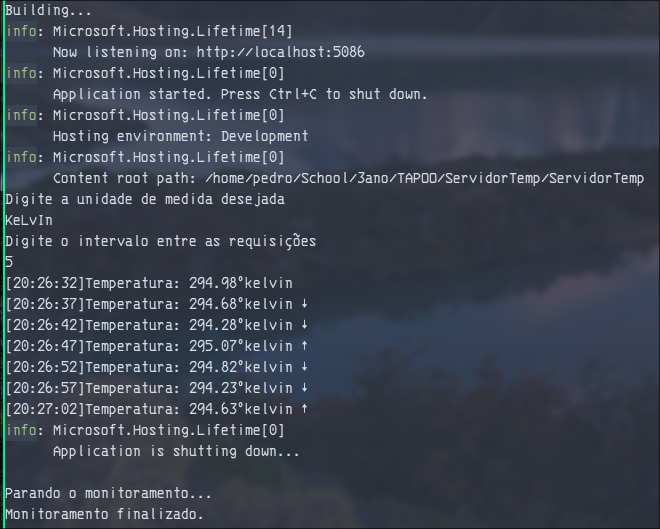
\includegraphics[width=1\textwidth]{imgs/img3.png}
    \caption{Execução do programa com unidade Kelvin}
    \label{fig:img3}
\end{figure}

\begin{figure}[H]
    \centering
    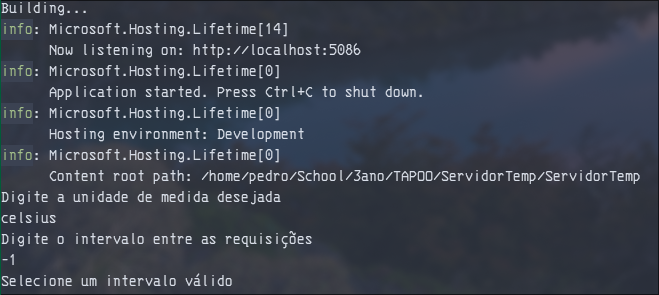
\includegraphics[width=1\textwidth]{imgs/img4.png}
    \caption{Tratamento de erro para intervalo inválido}
    \label{fig:img4}
\end{figure}

\begin{figure}[H]
    \centering
    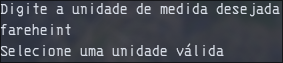
\includegraphics[width=1\textwidth]{imgs/img5.png}
    \caption{Tratamento de erro para unidade inválida}
    \label{fig:img5}
\end{figure}

\section{Conclusão}

Todos os objetivos do projeto foram alcançados com sucesso. O desenvolvimento do programa de monitoramento de temperatura proporcionou aprendizado prático sobre APIs REST, tanto na perspectiva de criação quanto de consumo.

Na criação de APIs REST, foi possível compreender como estruturar endpoints HTTP utilizando ASP.NET Core, definindo rotas parametrizadas e retornando dados em formato JSON. A implementação do servidor demonstrou a simplicidade de mapear URLs para funções que processam requisições e geram respostas padronizadas.

No consumo de APIs REST, o projeto evidenciou o uso do HttpClient para realizar requisições GET, o tratamento de respostas HTTP e a deserialização de JSON para objetos C#. A experiência mostrou a importância do gerenciamento adequado de recursos HTTP e do tratamento de erros de comunicação.

O trabalho consolidou conhecimentos fundamentais sobre comunicação entre aplicações através de protocolos HTTP, demonstrando como sistemas distribuídos podem trocar informações de forma estruturada e eficiente utilizando o padrão REST.

\end{document}
